% Results: synthetic experiments (generated from experiments/synthetic_limit.py,
% outputs in results/synthetic/). Numbers below are taken from the CSVs in this folder.
% TODO: align notation (Z, A, D, Y, num, s, gamma) with the method section.

\section{Synthetic experiments}
\label{sec:synthetic}

We first study the feasible-set approach on synthetic populations whose joint distribution
$p(z, a, d, y)$ is specified exactly. Because no sampling is involved, the true value of
every metric is known, and any gap between an estimate and the truth comes from the method
itself, not from estimation error. In all experiments the common variable $Z$ takes $K$
equally likely values $z_1, \dots, z_K$ with scores $\ell_z$ evenly spaced in $[-1, 1]$. The
protected attribute is binary, with
\[
  P(A = 1 \mid Z = z) = 0.5 + 0.45\, s\, \ell_z ,
\]
so the \emph{proxy strength} $s \in [0, 1]$ controls how much $Z$ reveals about $A$
($s = 0$: nothing). Decisions follow logistic models in $\ell_z$ plus a term $\gamma a$, the
\emph{direct effect} of $A$ beyond $Z$; when $\gamma = 0$, $D$ and $A$ are conditionally
independent given $Z$. Unless stated otherwise $K = 3$ and $\gamma = -0.6$. Only the two
margins $p(z, d)$ (or $p(z, d, y)$) and $p(z, a)$ are passed to the method. For each population
we use the finest grid size $\texttt{num} \in \{2, 3, 4, 5, 10, 20\}$ whose enumeration stays
below $2 \times 10^6$ joint distributions. Where the metric is linear or linear-fractional in
the joint, we compare against exact bounds from a linear program over the same feasible set.

\subsection{Comparing two classifiers}
\label{sec:synthetic-compare}

\begin{figure}[t]
  \centering
  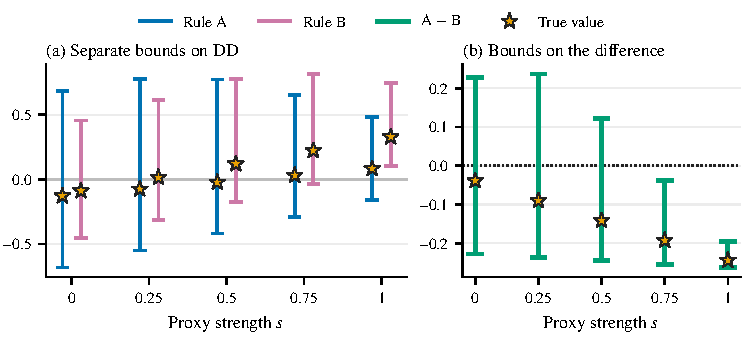
\includegraphics[width=\linewidth]{figures/synthetic_compare.pdf}
  \caption{Comparing two decision rules on the same population. (a) Bounds on the demographic
  disparity (DD) of each rule, computed separately. (b) Bounds on the difference
  $\mathrm{DD}(A) - \mathrm{DD}(B)$, computed from a single feasible set for the internal
  variable $(D_A, D_B)$. Stars mark the true values. $K = 3$, $\gamma = -0.6$,
  $\texttt{num} = 20$.}
  \label{fig:synthetic-compare}
\end{figure}

An auditor often wants to know whether one model is fairer than another, not only how fair
each one is. We construct two rules on the same population. Rule~A approves with probability
$\sigma(-0.2 + 0.8\,\ell_z + \gamma a)$. Rule~B approves everyone Rule~A approves, and also
80\% of Rule~A's denials in the upper half of the $Z$ bins. Treating the pair $(D_A, D_B)$ as a
single internal variable lets us bound the two DDs and their difference from one feasible
set.

Figure~\ref{fig:synthetic-compare} shows the result. Bounded separately, the two DD intervals
overlap at every proxy strength (panel a). From those intervals alone we cannot say which rule
has the smaller disparity, even at $s = 1$, where the intervals are
$[-0.16, 0.48]$ for A and $[0.10, 0.75]$ for B. The difference is far tighter, because the
same joint distribution has to explain both rules (panel b). Its width is $0.46$ at $s = 0$,
against $1.37$ and $0.91$ for the separate intervals. It shrinks to $0.07$ at $s = 1$, while
each separate interval is still $0.64$ wide. For $s \geq 0.75$ the interval on the difference
excludes zero, $[-0.25, -0.04]$ and $[-0.26, -0.20]$, which certifies that Rule~B has the
larger DD. Comparing the two separate intervals cannot reach this conclusion at any $s$. All grid bounds match the exact LP
bounds to numerical precision (differences below $10^{-12}$), as expected for metrics that are
linear in the joint.

\subsection{Bounding several metrics jointly}
\label{sec:synthetic-joint}

\begin{figure}[t]
  \centering
  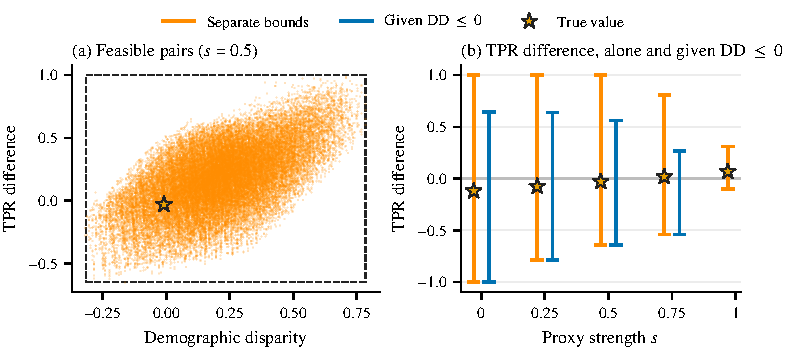
\includegraphics[width=\linewidth]{figures/synthetic_joint.pdf}
  \caption{Joint bounds on demographic disparity and the true positive rate (TPR) difference,
  with internal variable $(D, Y)$. (a) Feasible (DD, TPR difference) pairs at $s = 0.5$, with
  the box formed by the two separate intervals (dashed). (b) Bounds on the TPR difference alone,
  and restricted to joints with $\mathrm{DD} \le 0$. $K = 2$, $\texttt{num} = 10$.}
  \label{fig:synthetic-joint}
\end{figure}

With internal variable $(D, Y)$, every enumerated joint gives a value of both DD and the TPR
difference. This retains the dependence between the two metrics, which separate intervals
discard. Figure~\ref{fig:synthetic-joint}a shows the feasible pairs at $s = 0.5$. They fill an
elongated region, and across proxy strengths their convex hull covers only 57--63\% of the box
spanned by the two separate intervals. The two metrics are positively correlated over the
feasible set (correlation 0.47--0.68). Consequently, the upper-left and lower-right
corners of the box, such as a large negative DD together with a large positive TPR
difference, cannot occur.

One use of this structure is to combine side information about one metric with bounds on
another. Figure~\ref{fig:synthetic-joint}b restricts the feasible set to joints with
$\mathrm{DD} \le 0$. The upper bound on the TPR difference drops from $1.00$ to $0.64$ at
$s = 0$, from $1.00$ to $0.56$ at $s = 0.5$, and from $0.80$ to $0.27$ at $s = 0.75$. The lower
bound does not change, because the most negative TPR differences already occur at negative DD.
At $s = 1$ the margins rule out $\mathrm{DD} \le 0$ altogether (DD $\in [0.07, 0.27]$), so the
restricted set is empty.

\subsection{Sensitivity to conditional independence}
\label{sec:synthetic-sensitivity}

\begin{figure}[t]
  \centering
  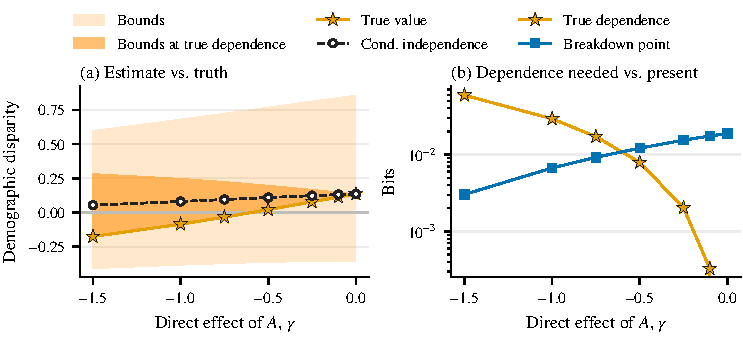
\includegraphics[width=\linewidth]{figures/synthetic_sensitivity.pdf}
  \caption{Departures from conditional independence. (a) True DD, the estimate under
  conditional independence (CI), the full bounds, and the bounds restricted to joints whose
  dependence $I(D; A \mid Z)$ is at most its true value. (b) The true dependence and the
  breakdown point, the least dependence at which the bounds reach the opposite sign from the
  CI estimate. $K = 3$, $s = 0.6$, $\texttt{num} = 100$.}
  \label{fig:synthetic-sensitivity}
\end{figure}

A common alternative to bounding is to assume $D \perp A \mid Z$ and report the resulting point
estimate. Here we vary the direct effect $\gamma$ from $0$ to $-1.5$ at fixed $s = 0.6$, so the
assumption holds exactly at $\gamma = 0$ and is increasingly violated as $\gamma$ moves away from
zero (Figure~\ref{fig:synthetic-sensitivity}a). The CI estimate is exact at $\gamma = 0$, but its
error grows steadily, reaching $0.23$ at $\gamma = -1.5$. The estimate also gets the sign wrong:
for $\gamma \le -0.75$ the true DD is negative ($-0.03$ to $-0.18$), while the CI estimate stays
positive ($0.09$ to $0.05$). The full bounds, roughly $[-0.36, 0.86]$ at $\gamma = 0$ and
$[-0.41, 0.60]$ at $\gamma = -1.5$, contain the truth throughout, but they are wide.

Each joint in the feasible set comes with its conditional dependence $I(D; A \mid Z)$, which
gives a middle ground between these two extremes. Restricting to joints with dependence at most
$\delta$ yields bounds that grow from the CI point ($\delta = 0$) to the full interval. At the
true dependence these bounds always contain the true DD and are much narrower than the full
bounds, e.g.\ $[-0.18, 0.28]$ at $\gamma = -1.5$ and $[0.02, 0.20]$ at $\gamma = -0.5$. The same
quantity gives a breakdown point: the least dependence at which DD can take the opposite sign
from the CI estimate (Figure~\ref{fig:synthetic-sensitivity}b). It decreases from $0.019$ bits at
$\gamma = 0$ to $0.003$ bits at $\gamma = -1.5$, because the CI estimate moves closer to zero.
Meanwhile, the true dependence increases from $0$ to $0.059$ bits. The two curves cross between
$\gamma = -0.5$ and $\gamma = -0.75$, exactly where the true DD changes sign. The breakdown point
therefore gives a correct test here: the sign of the CI estimate can be trusted when the true
dependence is below the breakdown point, and it is wrong when the true dependence is above it.
Bounds under a dependence constraint and the breakdown point are convex problems, so we also
solved them directly. The grid values agree closely with these solutions: the grid breakdown
point overestimates the exact one by at most 2.3\%, and the restricted bounds are inside the exact
ones by at most $0.003$.

\subsection{Computational cost and limits}
\label{sec:synthetic-cost}

\begin{figure*}[t]
  \centering
  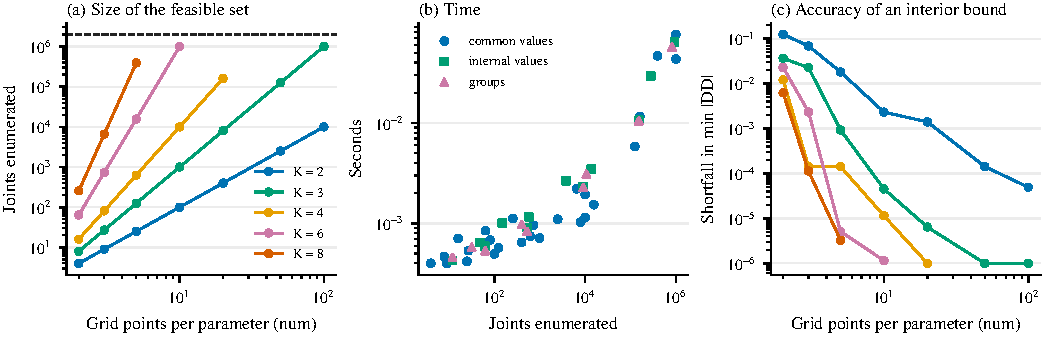
\includegraphics[width=\linewidth]{figures/synthetic_cost.pdf}
  \caption{Cost and accuracy of the grid. (a) Number of joints enumerated against grid size
  \texttt{num}, for $K$ common values (binary $D$ and $A$); the dashed line is the
  $2 \times 10^6$ cap. (b) Enumeration time against the number of joints, varying the number of
  common values, internal values and groups. (c) Shortfall of the grid's minimum $|\mathrm{DD}|$
  relative to the exact value (zero in every case), floored at $10^{-6}$.}
  \label{fig:synthetic-cost}
\end{figure*}

The approach enumerates a grid over the free cells of the joint table. With $K$ common values,
$B$ internal values and $G$ groups, there are $F = K(B-1)(G-1)$ free parameters, so the grid has
$\texttt{num}^F$ points. Figure~\ref{fig:synthetic-cost}a shows this growth. With binary $D$
and $A$, every grid point is feasible and the number of joints is exactly $\texttt{num}^K$. With
more internal values or groups, some combinations violate the margins, and 51--95\% of the grid
points are kept (e.g.\ $929{,}215$ of $10^6$ for $B = 4$, $\texttt{num} = 10$). Under the
$2 \times 10^6$ cap, the finest feasible grid is $\texttt{num} = 100$ for $K \le 3$, $20$ for
$K = 4$, $10$ for $K = 6$ and $5$ for $K = 8$. With $K = 2$ it is $20$, $10$ and $5$ for
$B = 3, 4, 5$, and $20$ and $10$ for $G = 3, 4$. The cost is therefore set by $F$, and the
approach suits problems with few common values, internal values and groups. Within that range it
is cheap. Time is roughly linear in the number of joints and does not depend on which dimension
produced them (Figure~\ref{fig:synthetic-cost}b). A million joints take under $0.1$\,s, and every
run in Sections~\ref{sec:synthetic-compare}--\ref{sec:synthetic-sensitivity} takes under
$0.1$\,s.

Bounds attained at a vertex of the feasible set (all bounds of linear metrics) are exact for
any \texttt{num}, because the Fréchet endpoints are always on the grid. Bounds attained in the
interior of the feasible set are only approximated. To measure this we use the minimum of
$|\mathrm{DD}|$, whose exact value is $0$ in every configuration
(Figure~\ref{fig:synthetic-cost}c). The shortfall falls quickly with \texttt{num}: from $0.12$ at
$\texttt{num} = 2$ to $5 \times 10^{-5}$ at $\texttt{num} = 100$ for $K = 2$, and below
$10^{-5}$ at the finest feasible grid for every $K \ge 3$. Larger $K$ gives a smaller shortfall
at the same \texttt{num}, because more combinations of cells are available to approach the
interior optimum. The shortfall need not decrease monotonically, however. Grids for different
\texttt{num} are not nested (for example, the grid for $\texttt{num} = 10$ does not contain the
midpoint used when $\texttt{num} = 3$ or $5$). For $B = 4$ the shortfall is $0$ at
$\texttt{num} = 3$ and $5$, but $0.007$ at $\texttt{num} = 10$. When interior bounds matter,
nested grid sizes (e.g.\ $\texttt{num} = 2^k + 1$) avoid this.

\paragraph{Summary.}
On populations with known ground truth, the feasible-set approach
(i)~recovers the exact bounds for linear metrics,
(ii)~gives conclusions from joint bounds that separate per-metric intervals cannot,
whether comparing two classifiers or combining two metrics,
(iii)~quantifies how much conditional dependence it takes to overturn a CI-based conclusion,
using a breakdown point that matched the true sign change in our experiment,
and (iv)~runs in well under a second when the number of free parameters is small. Its main
limitation is the exponential growth of the grid in $K(B-1)(G-1)$, which restricts it to coarse
proxies and few groups unless the common variable is binned.
